\chapter{Estrategias de planificación de queries}
\label{cap:epq}


\section{Predicción del tiempo de respuesta a \textit{queries} en un motor de búsqueda}
\label{scheduling:ptrq}
Conocer de antemano la eficiencia de una \textit{query} es una ventaja importante para usar técnicas efectivas de \textit{scheduling} de \textit{queries} en motores de búsqueda. Existen estudios en los cuales la eficiencia es inferida usando \textit{clarity score} \citep{Cronen-Townsend:2002}, que es una forma para evaluar la pérdida de ambigüedad de una query con respecto a la colección. En \citep{He:2004} se propone un conjunto de predictores para la eficiencia de cada \textit{query}. Técnicas de aprendizaje de máquina también han sido estudiadas para predecir la eficiencia de \textit{queries} \citep{Si:2002}. Todos los estudios mencionados anteriormente se han centrado en la efectividad para ser predicciones. La eficiencia también ha sido utilizada para predecir el tiempo de respuesta de una query, identificando las razones por las que ésta puede ser resuelta ineficientemente y evaluando estos factores para predecir el comportamiento de futuras queries \citep{Tonellotto:2011}.

En el predictor propuesto en \citep{Macdonald:2012} está basado en estadísticos  disponibles de los términos de la query. 

\begin{tabular}{|l|}
\hline 
Estadístico del término s(t) \\ 
\hline 
1. Media aritmética del score \\ 
\hline 
2. Media geométrica del score \\ 
\hline 
3. Media armonica del score \\ 
\hline 
4. Puntaje máximo \\ 
\hline 
5. Varianza de puntaje \\ 
\hline 
6.  \\ 
\hline 
Agregadores \\ 
\hline 
Máximo \\ 
\hline 
Varianza \\ 
\hline 
Suma \\ 
\hline 
\end{tabular} 


Este predictor está evaluado comparado con 10.000 queries == individual and combinated


\section{Wand \textit{multi-threaded}}
\label{scheduling:wm}
Dado que el método WAND \citep{Broder:2003} consiste en el método del estado del arte ocupado hoy en día por los motores de búsqueda, en esta investigación se asume un sistema que usa este método para obtener eficientemente los mejores K documentos a una transacción de lectura. Este algoritmo usa un \textit{ranking} basado en una evaluación de dos niveles. En el primer nivel, este usa una cota superior (\textit{upper bound}) al puntaje de cada documento para intentar descartarlos eficientemente. En el segundo nivel se computa el puntaje real de los documentos que pasa el primer nivel. Para hacer que este proceso trabaje eficientemente, se usa una estructura de datos llamada \textit{heap} que va guardando el conjunto de los mejores K documentos hasta determinado instante. El menor puntaje de este conjunto es usado como umbral para las evaluaciones del primer nivel, de esta forma se descarta rápidamente documentos que no pueden ser parte del conjunto final de los \textit{top-K} documentos. Esto permite un eficiente y a la vez seguro proceso de descarte que asegura que en el resultado final se encontrará el conjunto correcto y no se perderán documentos relevantes.

Existen dos formas de implementar WAND \textit{multithreaded}. Uno de ellos es usando \textit{heaps} locales (LH), es decir, un \textit{heap} por \textit{thread} y el otro es usando \textit{heaps} compartidos (SH). El estudio en \citep{Rojas:2013} se muestra indicios que el esquema SH es generalmente más eficiente. Logrando rápidamente un óptimo valor para el threshold, el esquema SH posee las siguientes ventajas: (1) Se puede reducir el número de calculo de puntajes completjos y (2) son ejecutadas pocas operaciones de actualización del heap (reduciendo el número de locks que se hace a la estructura de dato). A continuación se presenta el diseño llevado a cabo para ambos esquemas.


\subsection{Wand con heaps locales}
\label{scheduling:whl}
En el esquema LH, cada thread procesa una porción del índice invertido mientras mantiene un heap local con los mejores K documentos que el específico thread ha encontrado hasta ahora. Al final del proceso, el resultado de cada thread debe ser reunido en un solo conjunto final global. Los resultados en \citep{Rojas:2013} muestran que el esquema LH es más eficientes para aquellas transacciones que toman poco tiempo en ser resueltas. En la Figura \ref{fig:wand-heap-local} se muestra el esquema de ejecución para heaps locales explicado anteriormente. 

\begin{figure}[tp]
\centering
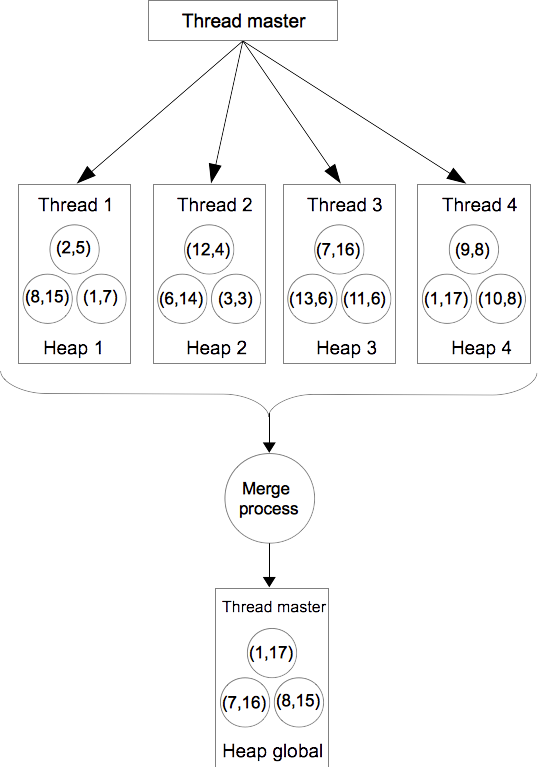
\includegraphics[scale=.75]{images/wand-heap-local.png}
\caption{Esquema de ejecución de algoritmo WAND con heaps locales}
\label{fig:wand-heap-local}
\end{figure}

El diseño aplicado para implementar el esquema LH se puede ver en la Figura \ref{fig:TopKMultiThreadWandOperatorLocal}. La clase principal es la TopKMultiThreadWandOperatorLocal, que es la encargada de controlar el paralelismo en la resolución de las transacciones. Para explicar de mejor manera cada una de las clases involucradas en la implementación, se presenta el siguiente diccionario de datos.

\begin{list}{}{}
	\item \textbf{TopKMultiThreadWandOperatorLocal}. Clase encargada de devolver los mejores K documentos para una query dada. Si es que la query debe ser resuelta en forma paralela, esta clase además debe controlar el paralelismo que se produce en la resolución de ésta, inicializando las variables correspondientes para lanzar los hilos de ejecución y luego escogiendo los mejores documentos desde todos los heaps creados por los diferentes threads (proceso de merge). En esta clase se define un mapa que asocia cada término del índice invertido con el puntaje del mejor documento en esa lista invertida (upper bound de la lista invertida) y además se define cuántos documentos se van a retornar al final del proceso (atributo K). El método execute inicializa las variables locales para los diferentes threads, posteriormente hace el llamado al método thread_execute (en el cual se llevará a cabo la resolución de la transacción de lectura en forma paralela), finalmente se toman los resultados parciales de cada uno de los hilos de ejecución y se ejecuta el proceso que mezcla los resultados, retornando solo los mejores K documentos. 
	
	\item \textbf{PartitionedInvertedIndex}. Clase que tiene la tarea de almacenar el índice invertido y extraer desde aquí las listas invertidas de documentos para cada uno de los términos de las transacciones de lectura. El almacenamiento el índice se lleva a cabo mediante un mapa cada término su lista invertida correspondiente y para la extracción de estas listas se usa el método getList.
	
	
	\item \textbf{TopKWandOperator}.  Cada thread tendrá su propio objeto TopKWandOperator encargado de obtener los mejores K documentos. El cálculo de este conjunto se realiza en el método execute con la ayuda de un objeto de tipo Wand asociado.
	
	\item \textbf{Wand}. Clase que controla la lógica del algoritmo wand. Lleva a cabo el proceso de inserción de documentos en el heap y todo lo que esto conlleva. 
	
	\item \textbf{ResultObject}. Clase que se utiliza para guardar los mejores K documentos.
	
	\item \textbf{QueryObject}. Clase que representa una transacción de lectura. Está constutuída sus términos,  las respectivas listas invertidas y pesos de cada uno de ellos, la cantidad de threads con los cuales se resolverá dicha transacción y el tiempo estimado de procesamiento (este tiempo se predice al momento de resolver la query).

\begin{figure}[H]
\centering
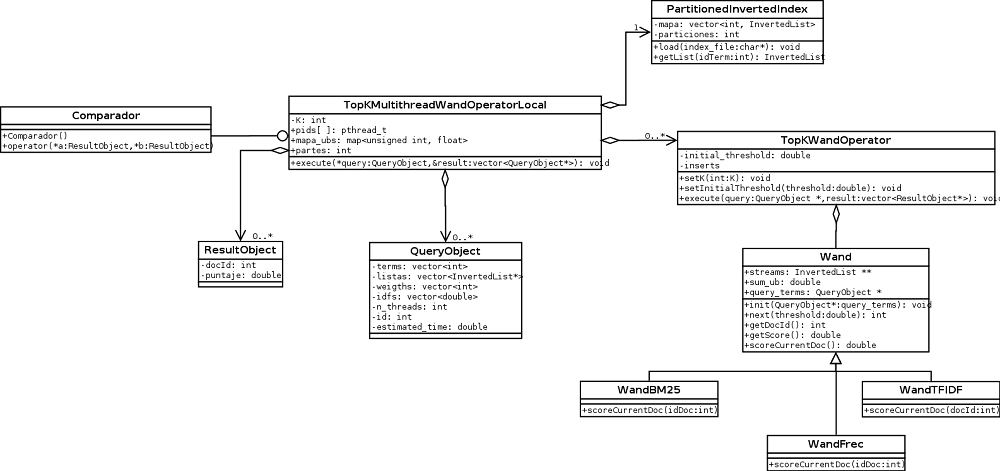
\includegraphics[scale=.75]{images/TopKMultiThreadWandOperatorLocal.png}
\caption{Diagrama de clases para el esquema LH}
\label{fig:TopKMultiThreadWandOperatorLocal}
\end{figure}


\subsection{Wand con heap compartido}
\label{scheduling:whc}
En el esquema SH cada thread procesa una perción del índice. Sin embargo, un solo heap es creado y accedido por todos los threads. En este caso no se requiere de mezcla y el proceso de descarte tiende a ser más eficiente porque los documentos con mayor puntaje tienden a estar en el heap. Sin embargo acceder al heap debe ser controlado por un lock o algún método similar que garantice el acceso exclusivo de los threads al heap.

\begin{figure}[H]
\centering
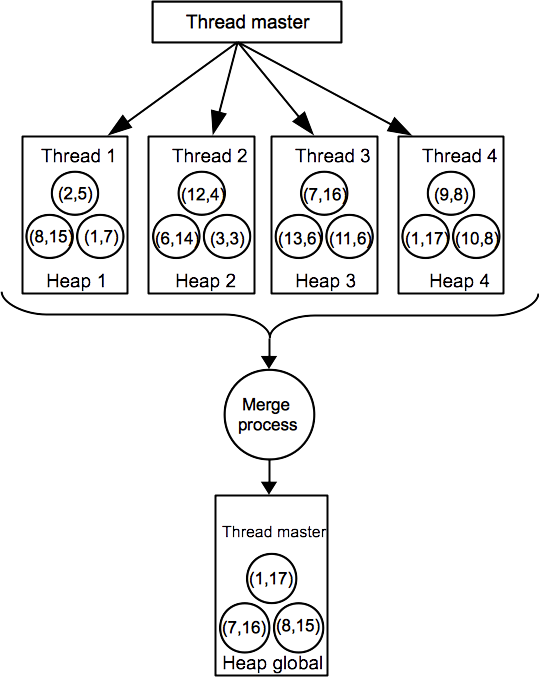
\includegraphics[scale=.75]{images/wand-heap-compartido.png}
\caption{Esquema de ejecución de algoritmo WAND con heap compartido}
\label{fig:wand-heap-compartido}
\end{figure}

\begin{figure}[H]
\centering
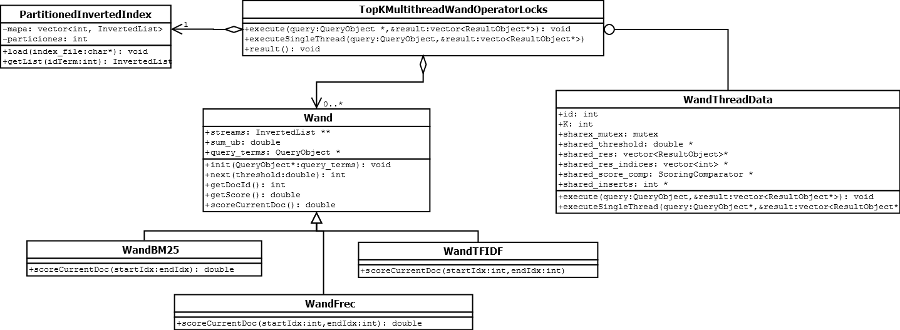
\includegraphics[scale=.75]{images/TopKMultiThreadWandOperatorLocks.png}
\caption{Diagrama de clases para el esquema SH}
\label{fig:TopKMultiThreadWandOperatorLocks}
\end{figure}






\section{Estrategia \textit{baseline}}
\label{scheduling:baseline}
Una simple manera de construir un sistema que responda a múltiple queries simultáneamente usando múltiple threads es, usando los threads de manera independiente. Para hacer esto, se debe mantener un conjunto de threads consumidores, cada uno de ellos se encargará de responder a queries secuencialmente y todos ellos trabajan en paralelo leyendo las queries desde la misma cola. Esto es lo que en este trabajo se denomina Un Thread Por Query (1TQ), ver Figura X (Profundizar más en esta figura)

Este esquema simple tiene ventajas y desventajas, además que es fácil de implementar y controlar. 

Existen sistemas que tienen que ejecutar un conjunto de queries de un cierto tamaño y luego parar para actualizar la información del índice invertido. Solo después de la fase de actualización, éste es capaz de ejecutar el siguiente conjunto de queries (batch de queries). Al final de cada batch, es posible que algunos threads finalicen su trabajo y que no tengan más queries para procesar, por lo que ellos tienen que esperar que los threads restantes finalicen su trabajo antes que el sistema entre en la fase de actualización. 

Sin embargo, aunque cada thread está secuencialmente ejecutando una query diferente, algunas de estas operaciones puede tomar un tiempo cosiderable, de esta forma se produce una importante pérdide de eficiencia, aunque la intuición nos dice que esto se puede amortizar con trabajos pequeños. Ver Figura 2 (Explicar)




\section{Estrategias de \textit{scheuling}}
\label{scheduling:es}
nosotros optamos por un enfoque de Wand Heap Compartido para ser usado en los experimentos.
\subsection{FR}
\label{scheduling:fr}

\subsection{Times}
\label{scheduling:times}

\subsection{TimesRanges}
\label{scheduling:timesranges}




\section{Estrategia de unidades de trabajo}
\label{scheduling:unidadestrabajo}